\documentclass{article}

\usepackage[hangul]{kotex} %<===> EUC-KR
\usepackage{ifxetex} % 부득이하게 pdflatex을 사용해도 문제가 없도록 함

\ifxetex
%한글 사용 옵션
\RequirePackage{xetexko}
\setmainfont[Ligatures=TeX]{Batang}
\setmainhangulfont[BoldFont=*,BoldFeatures=FakeBold,%
ItalicFont=*,ItalicFeatures=FakeSlant]{Batang}
\disablecjksymbolspacing
\nonfrenchspacing
\else
\fi

\usepackage{graphicx}
\usepackage{tikz}
\begin{document}


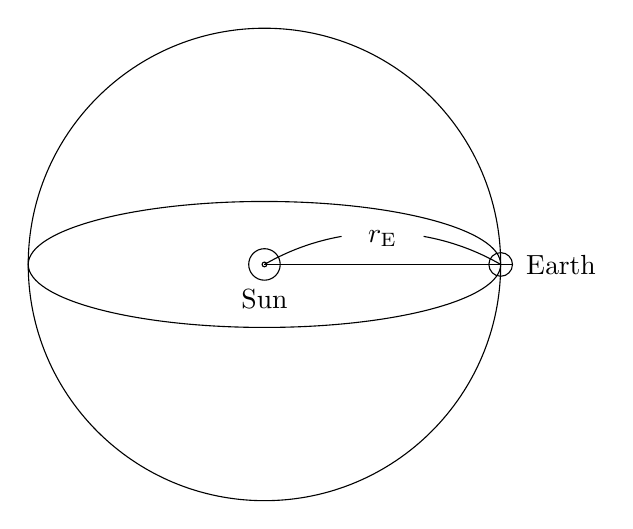
\begin{tikzpicture}[scale = 1, xshift = 1cm]
	\draw (5,2) circle (3cm);
	\draw (5,2) ellipse (3cm and 0.8cm);
	\draw (5,2) circle (0.03cm);
	\draw (5,2) circle (0.2cm) node[below, yshift=-0.2cm] {Sun};
	\draw (8,2) circle (0.15cm) node[right, xshift=0.2cm] {Earth};
	\draw (5,2) -- (8,2) node[above, xshift=-1.5cm, yshift=0.1cm] {$r_{\mathrm{E}}$};
	\draw (5,2) arc (120:100:3cm);
	\draw (8,2) arc (60:80:3cm);
	\draw (7.85,2) -- (8.15,2);
	\draw (8,1.85) -- (8,2.15);
\end{tikzpicture}


\end{document}